\documentclass[xcolor=table]{beamer}

% \rowcolors{1}{gray!30}{gray!10}

\usetheme{Boadilla}
\usecolortheme{dolphin}
\useoutertheme[subsection=false]{smoothbars}

\setbeamercolor{frametitle}{fg = black, bg = white} 
\setbeamercolor{palette primary}{use=structure,fg=white,bg=structure.fg!60!white}
\setbeamercolor{palette secondary}{use=structure,fg=white,bg=structure.fg!90!white}
\setbeamercolor{palette tertiary}{use=structure,fg=white,bg=structure.fg!120!white}
\setbeamercolor{palette quaternary}{use=structure,fg=black,bg=white} %Top bar

\setbeamertemplate{enumerate subitem}[circle]%
\renewcommand{\insertsubenumlabel}{\alph{enumii}}

\usepackage{amsmath}
\usepackage{xcolor}
\usepackage{booktabs}
\usepackage[utf8]{inputenc}
\usepackage{hyperref}
\usepackage[table]{xcolor}
\definecolor{lightgray}{gray}{0.9}

\hypersetup{
    colorlinks,
    citecolor=blue,
    linkcolor=blue
}

\footnotesize \let\small\footnotesize

\author{Jonathan P. Latner, PhD}
\title{Binary classification problem}
\date{\today}

\beamertemplatenavigationsymbolsempty 
\setbeamerfont{page number in head/foot}{size=\tiny}
\setbeamertemplate{footline}[frame number]
\setbeamertemplate{caption}[numbered]
\setbeamertemplate{section in toc}[sections numbered]

\begin{document}

\frame{\frametitle{ }
\titlepage
\thispagestyle{empty}
}

\section{Introduction}
\frame{\frametitle{Overview} 
\tableofcontents[hideallsubsections]
}

\frame{\frametitle{Goal} 

\begin{itemize}
    \item Explore both data sets, note down your key observations along with a kind of summary.
    \item Build a classifier – a prediction model based only on the training data, with the goal of achieving the best performance possible on the validation data.
    \item Visualize results and the work on this classification task.
\end{itemize}
}

\section{Summary statistics}

\frame{\frametitle{}
\begin{figure}
    \caption{Factor variables}
    \resizebox{.9\textwidth}{!}{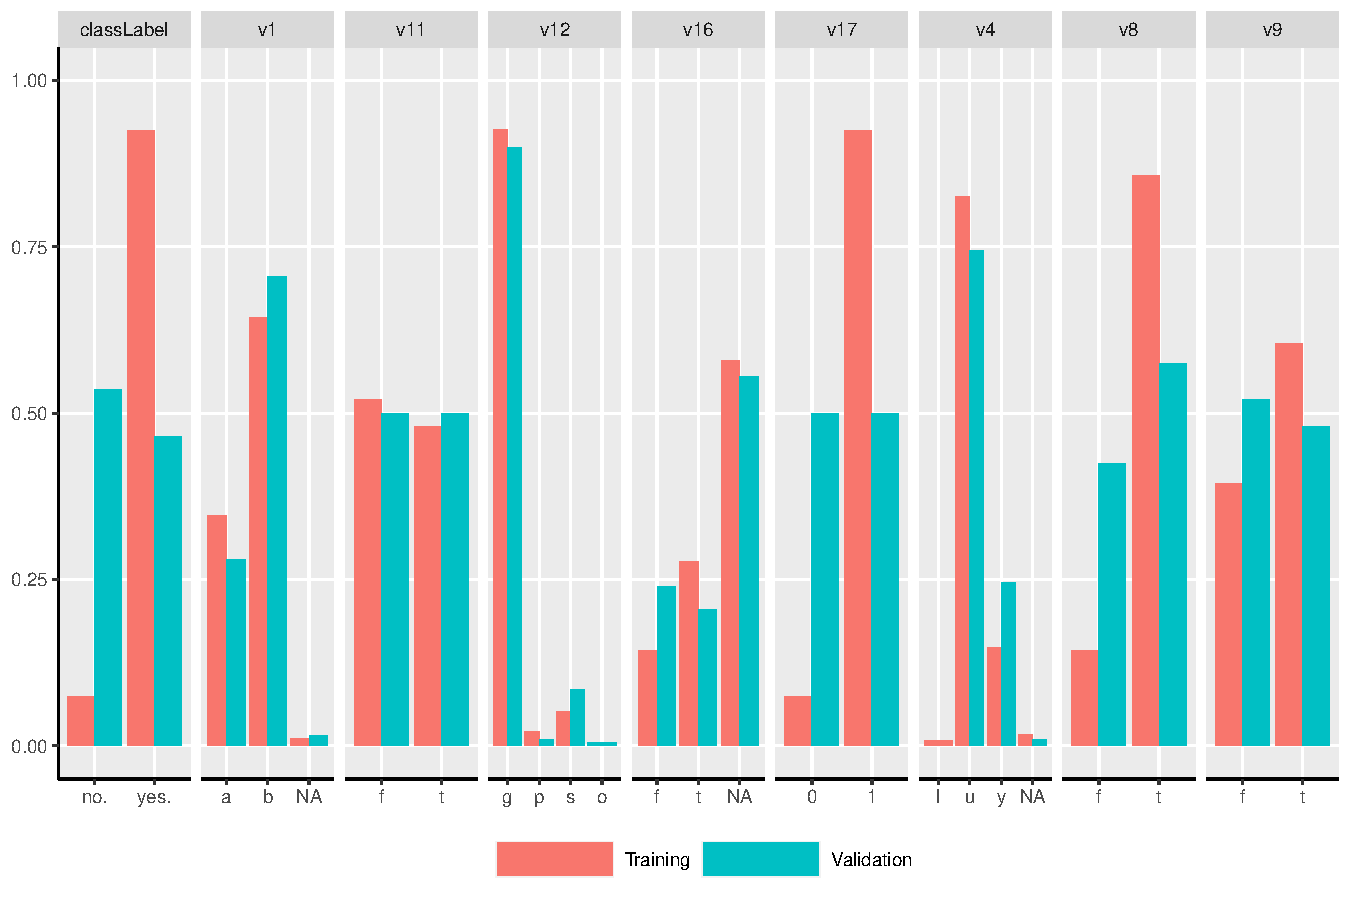
\includegraphics{../graphs/graph_vars_fctr.pdf}}
    \label{graph_vars_fctr}
\end{figure}
}

\frame{\frametitle{}
\begin{figure}
    \caption{Factor variables (correlation)}
    \resizebox{.9\textwidth}{!}{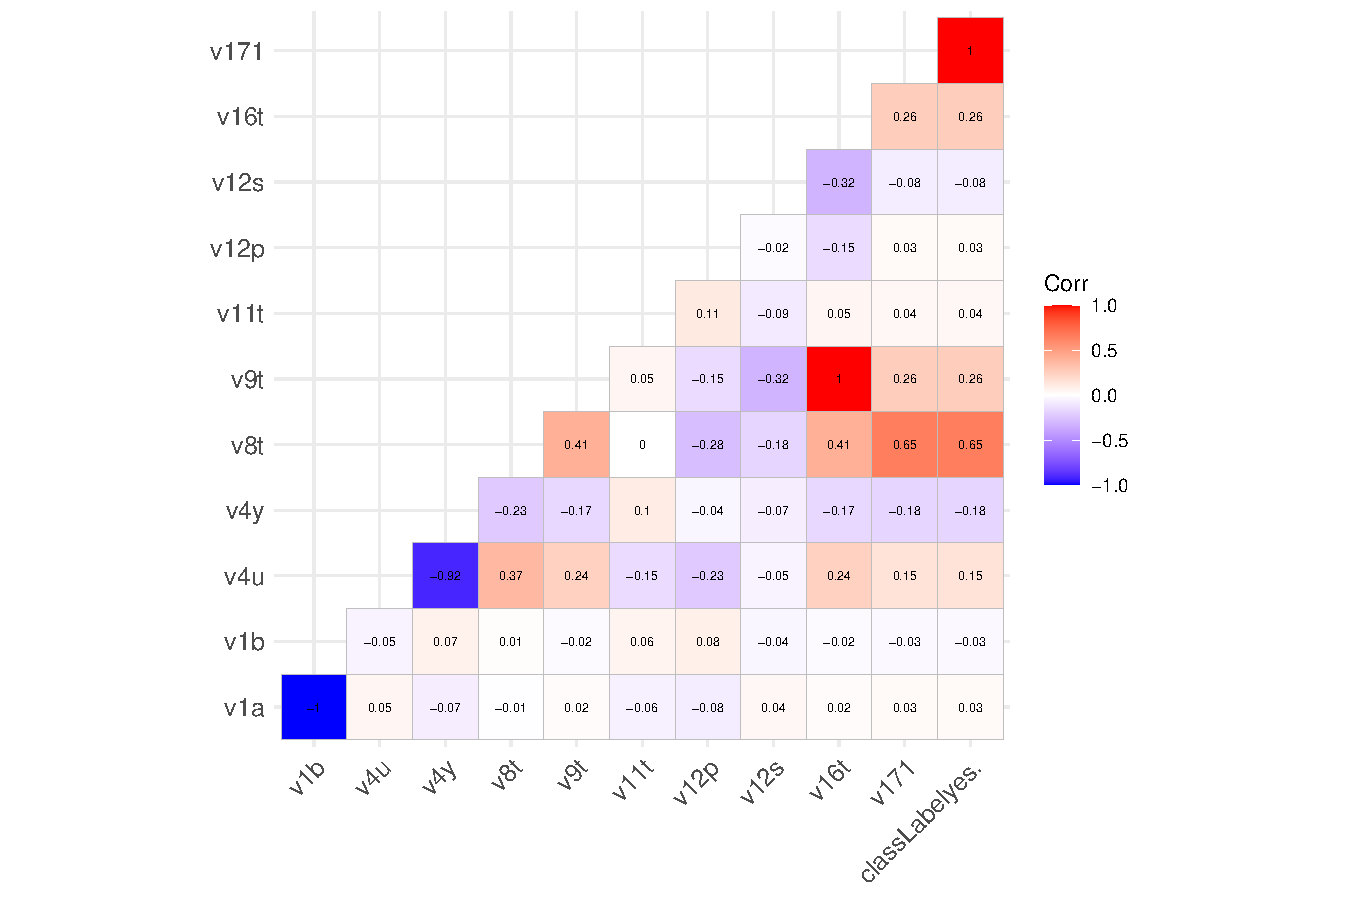
\includegraphics{../graphs/graph_corrplot_fctr.pdf}}
    \label{graph_corrplot_fctr.pdf}
\end{figure}
}


\frame{\frametitle{}
\begin{figure}
    \caption{Numerical variables}
    \resizebox{.9\textwidth}{!}{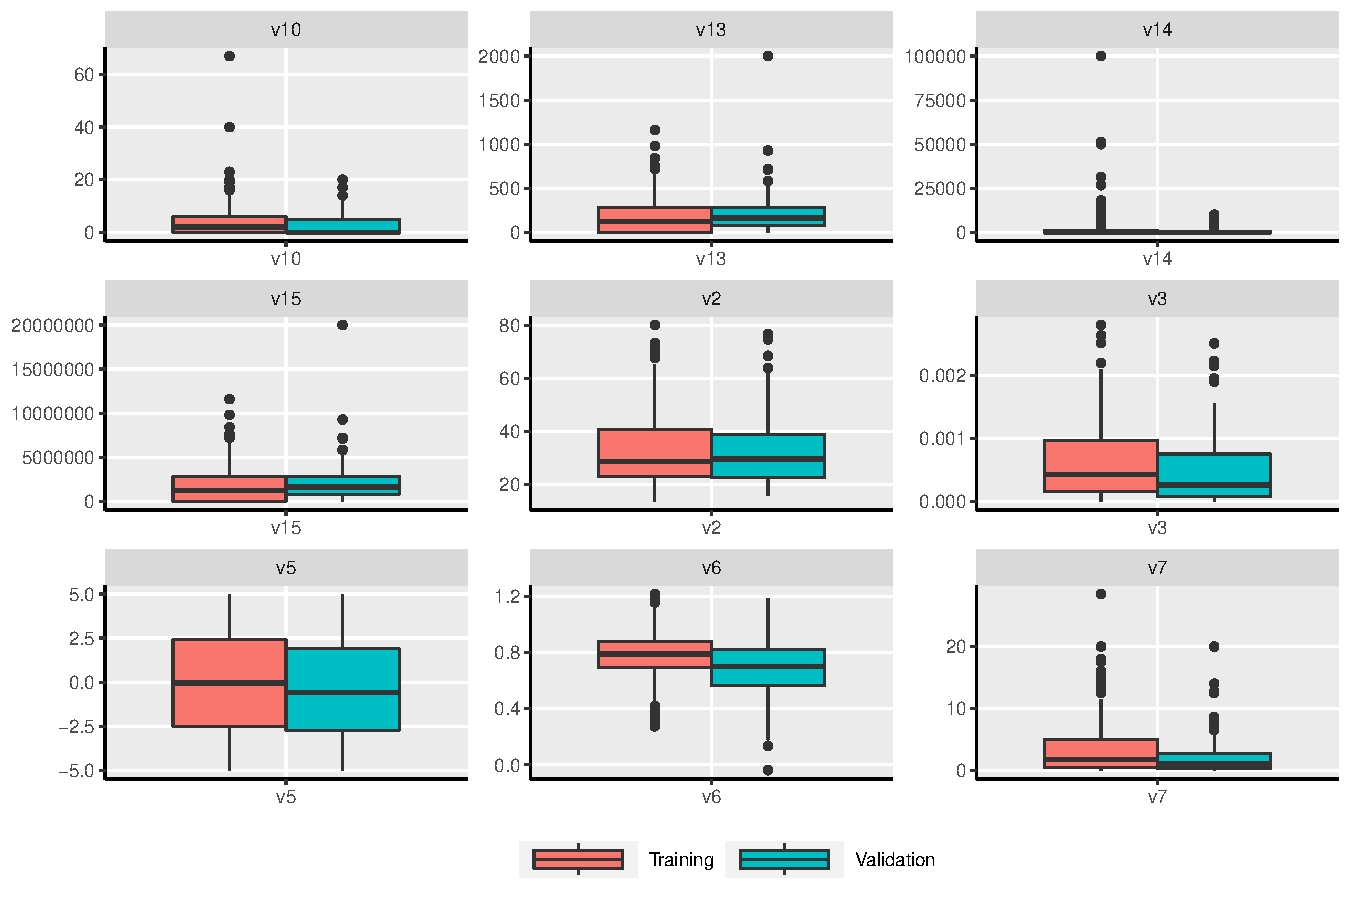
\includegraphics{../graphs/graph_vars_num.pdf}}
    \label{graph_vars_num}
\end{figure}
}

\frame{\frametitle{}
\begin{figure}
    \caption{Numerical variables (correlation)}
    \resizebox{.9\textwidth}{!}{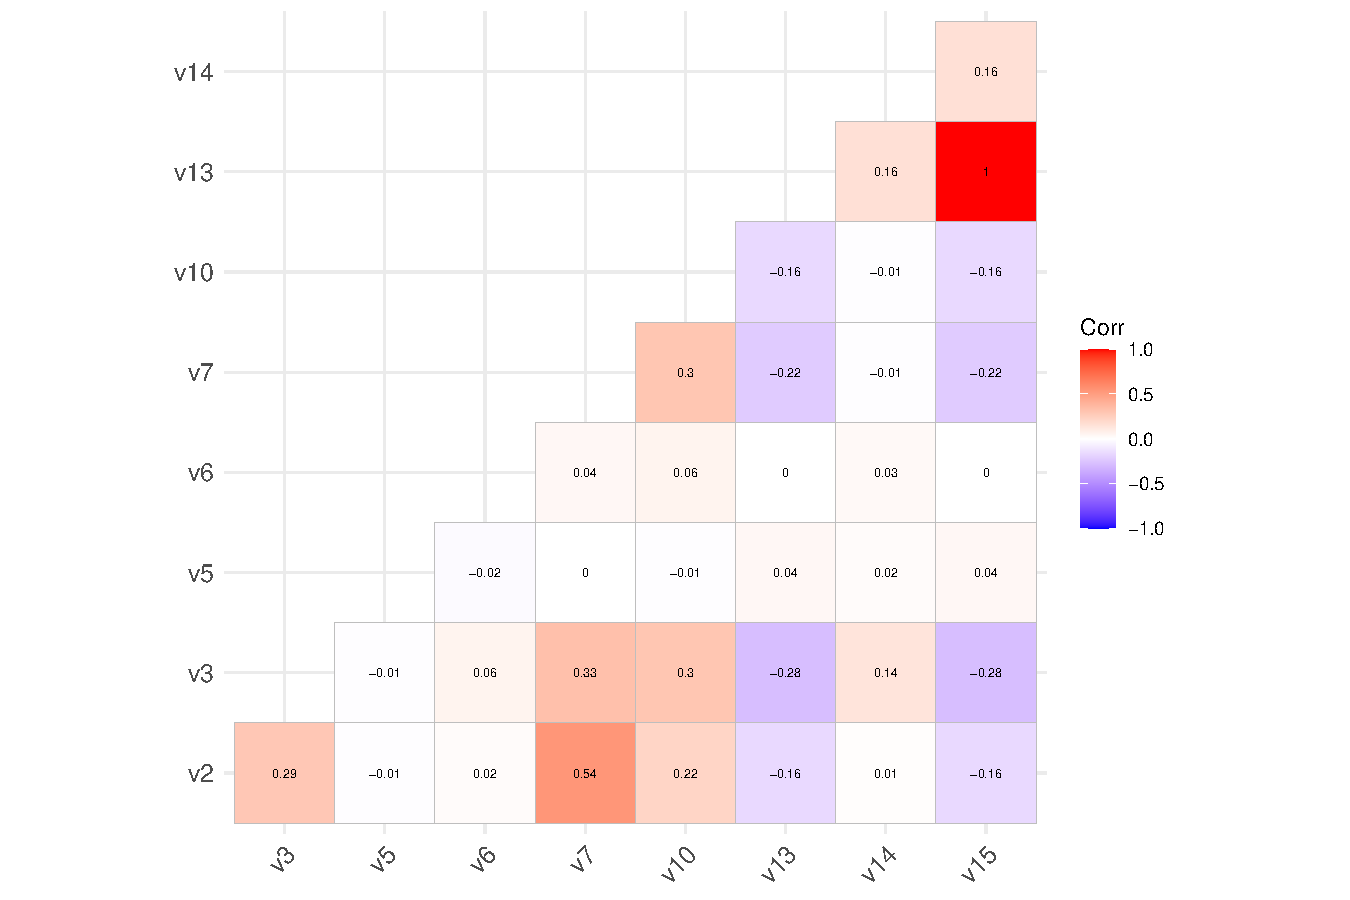
\includegraphics{../graphs/graph_corrplot_num.pdf}}
    \label{graph_corrplot_num}
\end{figure}
}

\frame{\frametitle{}
\begin{figure}
    \caption{Numerical variables (missing)}
    \resizebox{.9\textwidth}{!}{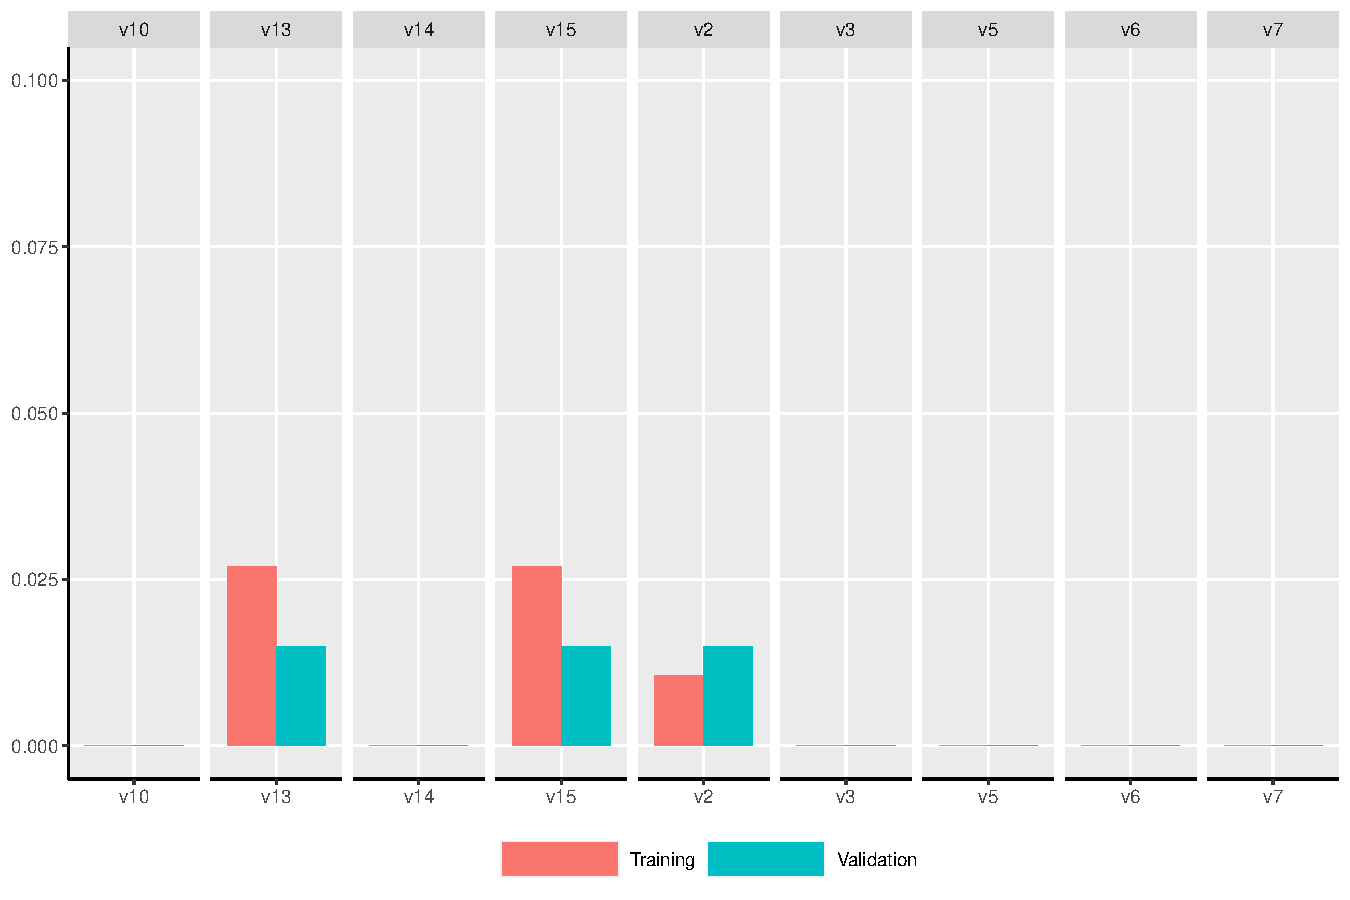
\includegraphics{../graphs/graph_vars_num_msng.pdf}}
    \label{graph_vars_num_msng}
\end{figure}
}

\frame{\frametitle{Initial lessons}
\begin{itemize}
    \item Classlabel (dv)
    \begin{itemize}
        \item v17 $=$ classLabel: keep classLabel, drop v17
        \item Difference in distribution between training and validation data
        \item Questionable power to predict 0/no, given low count in training data
    \end{itemize}
    \item v3 has mean, median, mode, and sd of 0, drop v3
    \item v12 training data has no "o"
    \item v4 validation data has no "l"
    \item v14 and especially v15 have a very long tail
    \item v13 and v15 perfectly correlated, drop v15
    \item Variable v16
    \begin{itemize}
        \item v9 and v16 are perfectly correlated (non missings)
        \item v16 has lots of missing observations (but missing in both traning and validation data)
        \item or is v9, v16 without any missing?
        % \item Steps to handle missing data in v16 in validation data
        % \begin{itemize}
        %     \item Assume all missings are ``f''
        %     \item Assume all missings are ``t''
        %     \item Assume random and even distribution of variable values (50/50)
        %     \item Assume missings follow distribution of variable values in training (39/61)
        % \end{itemize}
    \end{itemize}
\end{itemize}
}

\section{Model 1: Compare}
\frame{\frametitle{Steps} 
\begin{itemize}
    \item Compare different models with all IVs
    \begin{itemize}
        \item a) GLM
        \item b) Decision tree
        \item c) Random forest
        \item d) Naive Bayes
    \end{itemize}
    \item Examine model fit, summary statistics, etc.
\end{itemize}
}

\frame{\frametitle{Confusion matrix} 
\begin{table}[!h]
    % \caption{Model 1}
    \begin{center}
    \begin{tabular}{llrr}
   \toprule 
 & & \multicolumn{2}{l}{Model 1a: GLM} 
                        \\ 
 \cmidrule(lr){3-4} 
                        
  reality & predicted & 
                        Freq & Pct 
                        \\ \hline \\[-1.8ex]  
 0 & 0 &  49 & 0.91 \\ 
  1 & 0 &   5 & 0.09 \\ 
  0 & 1 &  50 & 0.37 \\ 
  1 & 1 &  86 & 0.63 \\ 
   \hline \\[-1.8ex]  

                   \multicolumn{2}{l}{Accuracy} & 
                   \multicolumn{2}{c}{0.711}
                   \\ 
 
                   \multicolumn{2}{l}{Duration (secs)} & 
                   \multicolumn{2}{c}{2.06}
                   \\ 
 \bottomrule 
\end{tabular}

    \label{table_model_01_cm}
    \end{center}
\end{table}
}

\frame{\frametitle{} 
\begin{table}[!h]
    \caption{Parameter estimates from logistic regression model 1a}
    \begin{center}
    \resizebox{.35\textwidth}{!}{
\begin{tabular}{l c}
\toprule
 & Model 1 \\
\midrule
(Intercept)    & $7.85 \;  (838.37)$        \\
v1b            & $0.02 \;    (0.23)$        \\
v2             & $-0.04 \;    (0.01)^{***}$ \\
v4u            & $-15.33 \;  (838.37)$      \\
v4y            & $-15.68 \;  (838.37)$      \\
v5             & $0.03 \;    (0.03)$        \\
v6             & $11.99 \;    (0.90)^{***}$ \\
v7             & $0.16 \;    (0.05)^{**}$   \\
v8t            & $3.58 \;    (0.24)^{***}$  \\
v9t            & $-0.91 \;    (0.33)^{**}$  \\
v10            & $0.28 \;    (0.08)^{***}$  \\
v11t           & $0.29 \;    (0.21)$        \\
v12p           & $-14.86 \; (1214.23)$      \\
v12s           & $-0.33 \;    (0.34)$       \\
v13            & $0.00 \;    (0.00)$        \\
v14            & $0.00 \;    (0.00)$        \\
\midrule
Log Likelihood & $-359.09$                  \\
Num. obs.      & $3523$                     \\
\bottomrule
\multicolumn{2}{l}{\scriptsize{$^{***}p<0.001$; $^{**}p<0.01$; $^{*}p<0.05$}}
\end{tabular}
}
    \label{glm_model_01}
    \end{center}
\end{table}
}

\frame{\frametitle{}
\begin{figure}
    \caption{Variable importance}
    \resizebox{.9\textwidth}{!}{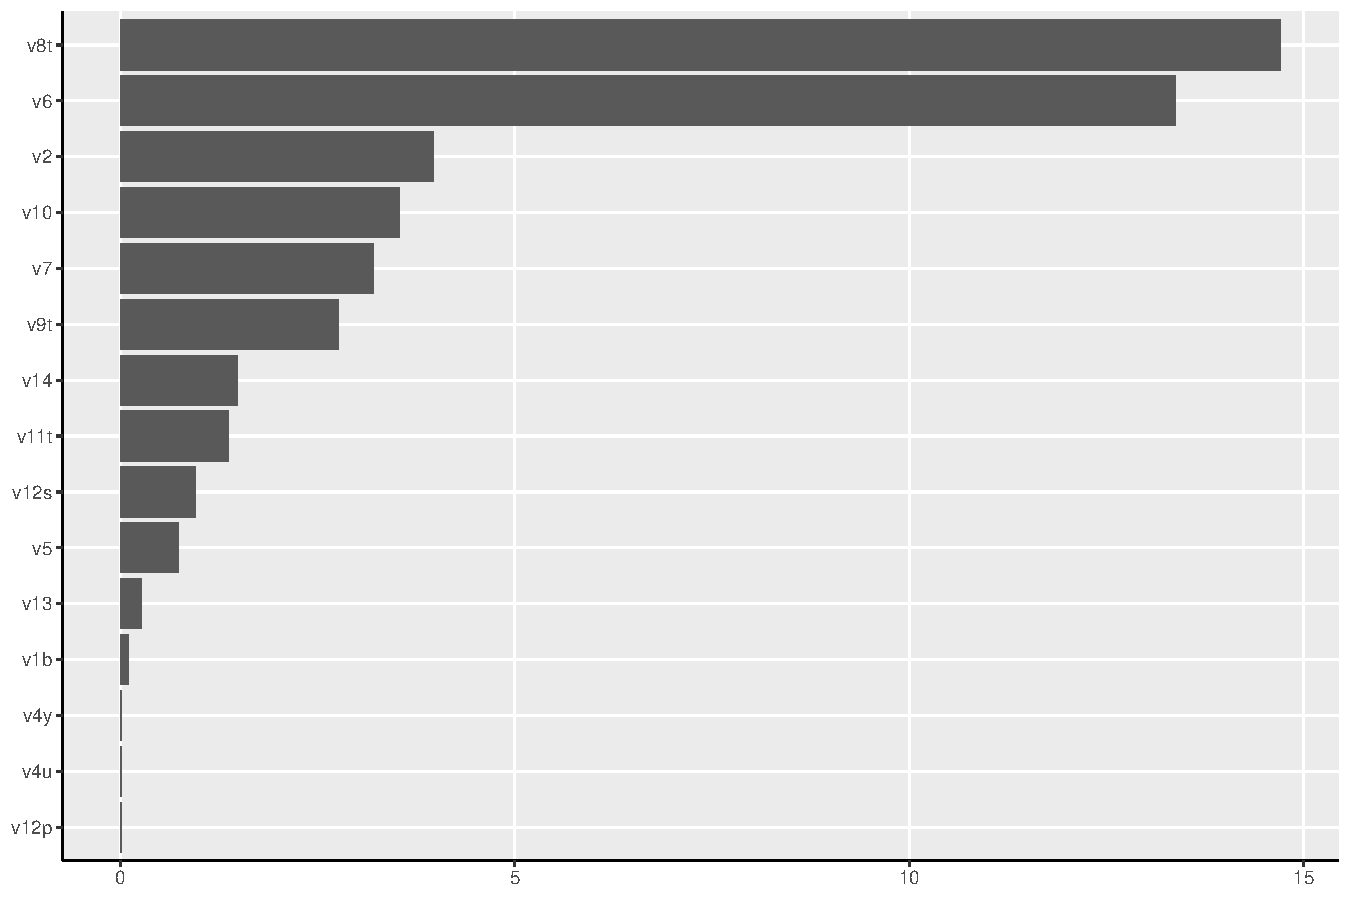
\includegraphics{../graphs/graph_model_01_importance.pdf}}
    \label{graph_model_01_importance}
\end{figure}
}

\frame{\frametitle{Lessons from model GLM} 
\begin{itemize}
    \item Decent model fit
    \begin{itemize}
        \item Good at predicting 0
        \item Bad at predicting 1
    \end{itemize}
    \item Drop variables?
    \begin{itemize}
        \item Categorical - v1, v4, combine v12s/v12p
        \item Continuous - v13, v14
    \end{itemize}
\end{itemize}
}

\frame{\frametitle{Add decision tree} 
\begin{table}[!h]
    \begin{center}
    \begin{tabular}{llrrrr}
   \toprule 
 & & \multicolumn{2}{l}{Model 1a: GLM} & 
                        \multicolumn{2}{l}{Model 1b: Tree} 
                        \\ 
 \cmidrule(lr){3-4} 
                        \cmidrule(lr){5-6} 
                        
  reality & predicted & 
                        Freq & Pct & 
                        Freq & Pct 
                        \\ \hline \\[-1.8ex]  
 0 & 0 &  49 & 0.91 &  51 & 0.96 \\ 
  1 & 0 &   5 & 0.09 &   2 & 0.04 \\ 
  0 & 1 &  50 & 0.37 &  48 & 0.35 \\ 
  1 & 1 &  86 & 0.63 &  89 & 0.65 \\ 
   \hline \\[-1.8ex]  

                   \multicolumn{2}{l}{Accuracy} & 
                   \multicolumn{2}{c}{0.711} & 
                   \multicolumn{2}{c}{0.737}
                   \\ 
 
                   \multicolumn{2}{l}{Duration (secs)} & 
                   \multicolumn{2}{c}{2.06} &
                   \multicolumn{2}{c}{2.05}
                   \\ 
 \bottomrule 
\end{tabular}

    \label{table_model_02_cm}
    \end{center}
\end{table}
}

\frame{\frametitle{Lessons from model 2} 
\begin{itemize}
    \item Slightly better fit
    \item Slightly better at predicting 0 (model 1 already good)
    \item Slightly better, but still bad at predicting 1
\end{itemize}
}

\frame{\frametitle{Add random forest} 
\begin{table}[!h]
    \begin{center}
    \resizebox{.75\textwidth}{!}{\begin{tabular}{llrrrrrr}
   \toprule 
 & & 
                        \multicolumn{2}{l}{Model 1a: GLM} & 
                        \multicolumn{2}{l}{Model 1b: Tree} & 
                        \multicolumn{2}{l}{Model 1c: RF} 
                        \\ 
 \cmidrule(lr){3-4} 
                        \cmidrule(lr){5-6} 
                        \cmidrule(lr){7-8} 
                        
  reality & predicted & 
                        Freq & Pct & 
                        Freq & Pct & 
                        Freq & Pct 
                        \\ \hline \\[-1.8ex]  
 0 & 0 &  49 & 0.91 &  51 & 0.96 &  72 & 0.95 \\ 
  1 & 0 &   5 & 0.09 &   2 & 0.04 &   4 & 0.05 \\ 
  0 & 1 &  50 & 0.37 &  48 & 0.35 &  27 & 0.24 \\ 
  1 & 1 &  86 & 0.63 &  89 & 0.65 &  87 & 0.76 \\ 
   \hline \\[-1.8ex]  

              \multicolumn{2}{l}{Accuracy} & 
                   \multicolumn{2}{c}{0.711} & 
                   \multicolumn{2}{c}{0.737} & 
                   \multicolumn{2}{c}{0.837}
                   \\ 
 
                   \multicolumn{2}{l}{Duration (secs)} & 
                   \multicolumn{2}{c}{2.06} &
                   \multicolumn{2}{c}{2.05} &
                   \multicolumn{2}{c}{65.47}
                   \\ 
 \bottomrule 
\end{tabular}
}
    \label{table_model_03_cm}
    \end{center}
\end{table}
}

\frame{\frametitle{Add naive bayes} 
\begin{table}[!h]
    \begin{center}
    \resizebox{.75\textwidth}{!}{\begin{tabular}{llrrrrrrrr}
   \toprule 
 & & 
                        \multicolumn{2}{l}{Model 1a: GLM} & 
                        \multicolumn{2}{l}{Model 1b: Tree} & 
                        \multicolumn{2}{l}{Model 1c: RF} &
                        \multicolumn{2}{l}{Model 1d: NB} 
                        \\ 
 \cmidrule(lr){3-4} 
                        \cmidrule(lr){5-6} 
                        \cmidrule(lr){7-8} 
                        \cmidrule(lr){9-10} 
                        
  reality & predicted & 
                        Freq & Pct & 
                        Freq & Pct & 
                        Freq & Pct & 
                        Freq & Pct 
                        \\ \hline \\[-1.8ex]  
 0 & 0 &  49 & 0.91 &  51 & 0.96 &  72 & 0.95 &  41 & 0.98 \\ 
  1 & 0 &   5 & 0.09 &   2 & 0.04 &   4 & 0.05 &   1 & 0.02 \\ 
  0 & 1 &  50 & 0.37 &  48 & 0.35 &  27 & 0.24 &  58 & 0.39 \\ 
  1 & 1 &  86 & 0.63 &  89 & 0.65 &  87 & 0.76 &  90 & 0.61 \\ 
   \hline \\[-1.8ex]  

              \multicolumn{2}{l}{Accuracy} & 
                   \multicolumn{2}{c}{0.711} & 
                   \multicolumn{2}{c}{0.737} & 
                   \multicolumn{2}{c}{0.837} & 
                   \multicolumn{2}{c}{0.689} 
                   \\ 
 
                   \multicolumn{2}{l}{Duration (secs)} & 
                   \multicolumn{2}{c}{2.06} &
                   \multicolumn{2}{c}{2.05} &
                   \multicolumn{2}{c}{65.47} &
                   \multicolumn{2}{c}{18.82}
                   \\ 
 \bottomrule 
\end{tabular}
}
    \label{table_model_04_cm}
    \end{center}
\end{table}
}

\frame{\frametitle{Summary} 
\begin{itemize}
    \item Random forest regression offers best fit
    \item Also much, much slower (time/energy costs money)
    \item Next steps: improve the model
\end{itemize} 
}

\section{Model 2: Forest}
\frame{\frametitle{Steps}
\begin{itemize}
    \item Begin with random forest baseline (all IVs, same as model 1c)
    \item Examine model fit, summary statistics, etc.
    \item Make adjustments
    \item Rerun model
    \item Repeat as necessary
\end{itemize} 
}

\frame{\frametitle{Confusion matrix} 
\begin{table}[!h]
    \begin{center}
    \resizebox{.5\textwidth}{!}{\begin{tabular}{llrr}
   \toprule 
 & & 
                        \multicolumn{2}{l}{Model 2a: Base} 
                        \\ 
 \cmidrule(lr){3-4} 
                        
  reality & predicted & 
                        Freq & Pct 
                        \\ \hline \\[-1.8ex]  
 0 & 0 &  71 & 0.95 \\ 
  1 & 0 &   4 & 0.05 \\ 
  0 & 1 &  28 & 0.24 \\ 
  1 & 1 &  87 & 0.76 \\ 
   \hline \\[-1.8ex]  

              \multicolumn{2}{l}{Accuracy} & 
                   \multicolumn{2}{c}{0.832}
                   \\ 
 
                   \multicolumn{2}{l}{Duration (secs)} & 
                   \multicolumn{2}{c}{93.49}
                   \\ 
 \bottomrule 
\end{tabular}
}
    \label{table_rf_model_rf_01_cm}
    \end{center}
\end{table}
}

\frame{\frametitle{}
\begin{figure}
    \caption{Variable importance}
    \resizebox{.9\textwidth}{!}{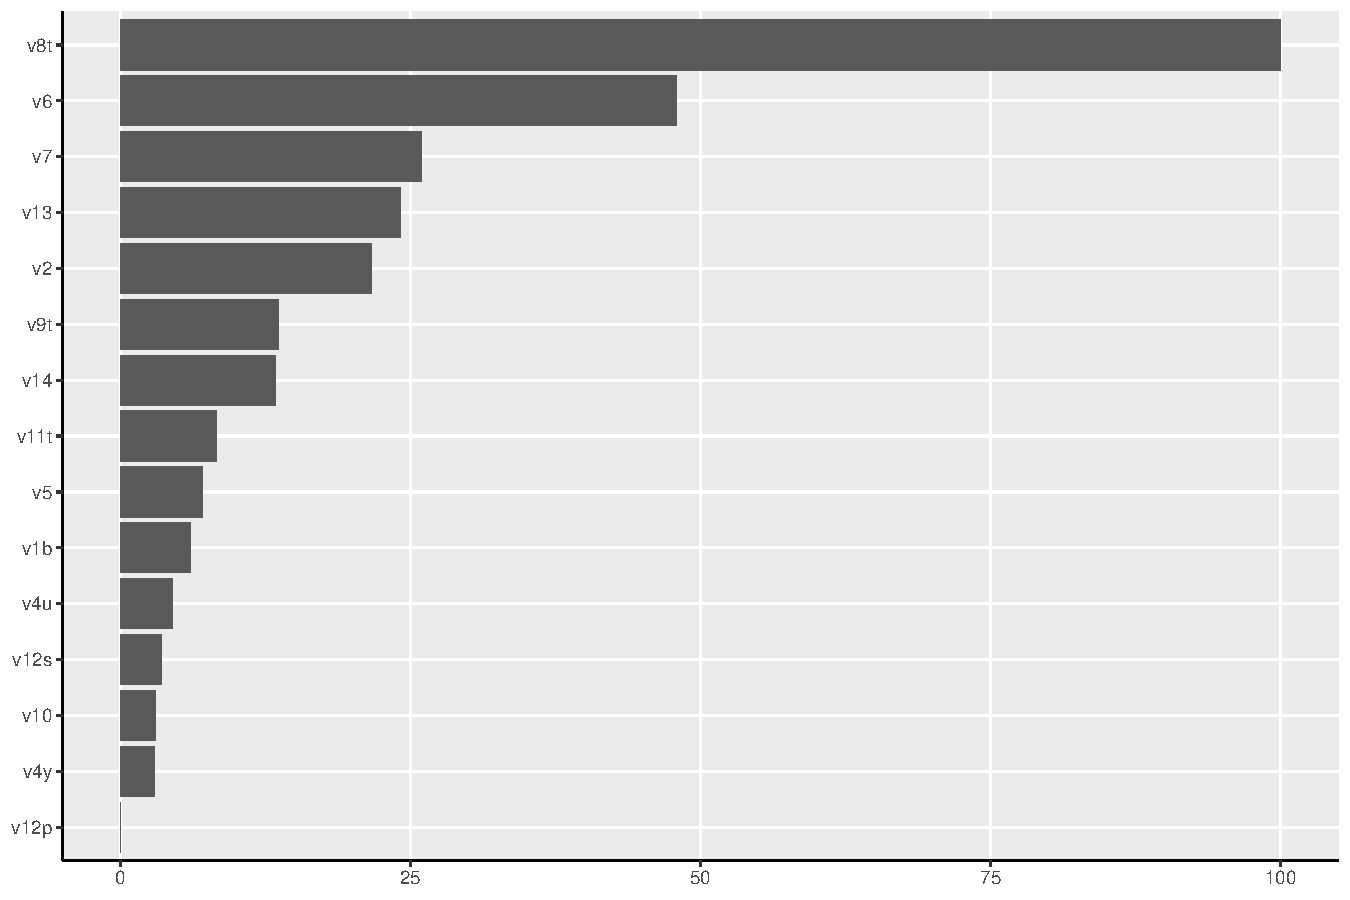
\includegraphics{../graphs/graph_model_rf_01_importance.pdf}}
    \label{graph_model_rf_01_importance}
\end{figure}
}

\frame{\frametitle{Lessons} 
\begin{itemize}
    \item Combine v12s/v12p
\end{itemize} 
}

\frame{\frametitle{Confusion matrix} 
\begin{table}[!h]
    \begin{center}
    \resizebox{.75\textwidth}{!}{\begin{tabular}{llrrrr}
   \toprule 
 & & 
                        \multicolumn{2}{l}{Model 2a: Base} &
                        \multicolumn{2}{l}{Model 2b: v12} 
                        \\ 
 \cmidrule(lr){3-4} 
                        \cmidrule(lr){5-6} 
                        
  reality & predicted & 
                        Freq & Pct &
                        Freq & Pct 
                        \\ \hline \\[-1.8ex]  
 0 & 0 &  71 & 0.95 &  69 & 0.96 \\ 
  1 & 0 &   4 & 0.05 &   3 & 0.04 \\ 
  0 & 1 &  28 & 0.24 &  30 & 0.25 \\ 
  1 & 1 &  87 & 0.76 &  88 & 0.75 \\ 
   \hline \\[-1.8ex]  

              \multicolumn{2}{l}{Accuracy} & 
                   \multicolumn{2}{c}{0.832} &
                   \multicolumn{2}{c}{0.826}
                   \\ 
 
                   \multicolumn{2}{l}{Duration (secs)} & 
                   \multicolumn{2}{c}{93.49} &
                   \multicolumn{2}{c}{82.03}
                   \\ 
 \bottomrule 
\end{tabular}
}
    \label{table_rf_model_rf_02_cm}
    \end{center}
\end{table}
}

\frame{\frametitle{}
\begin{figure}
    \caption{Variable importance}
    \resizebox{.9\textwidth}{!}{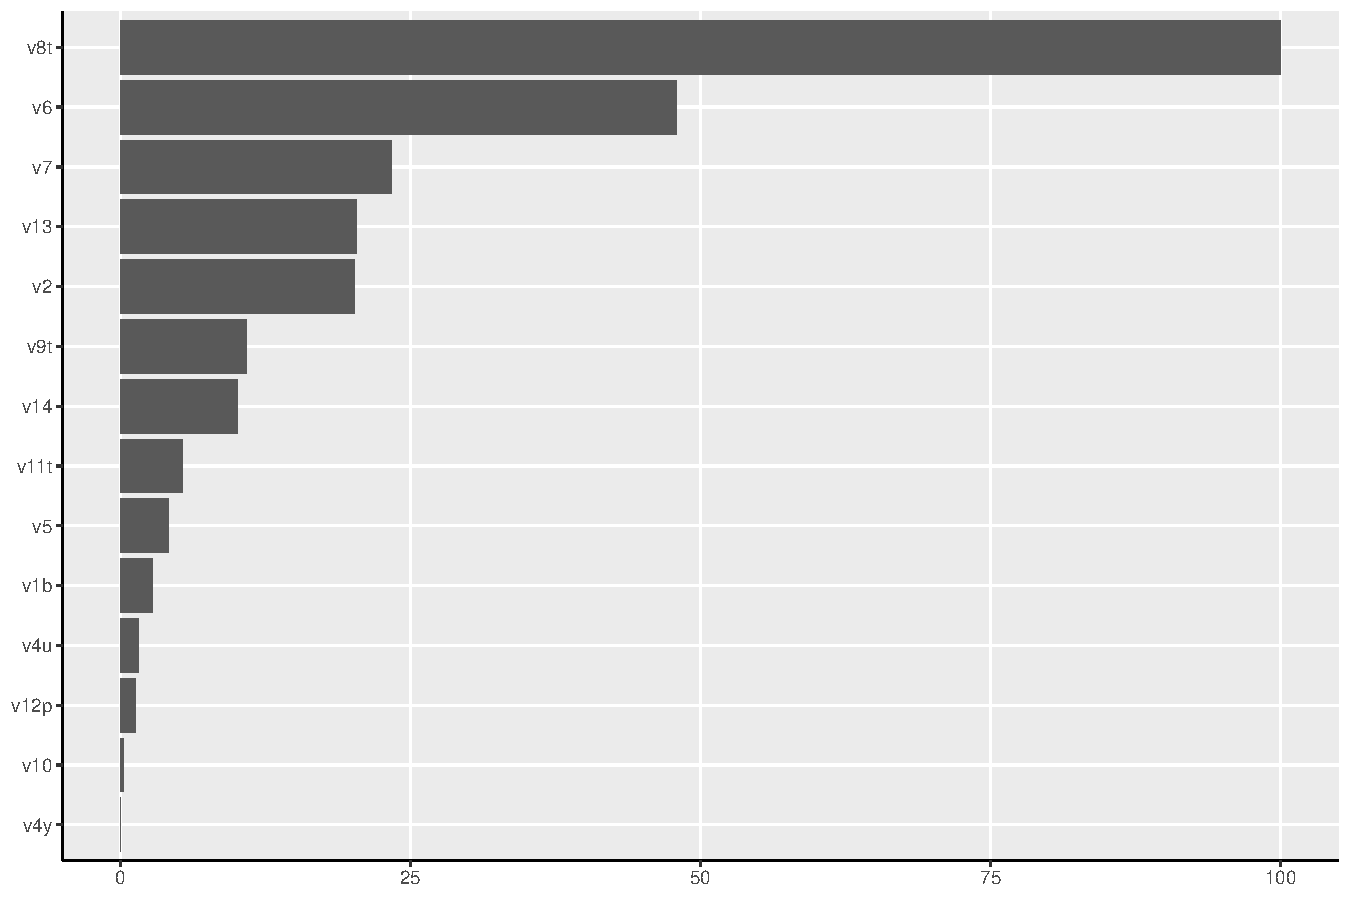
\includegraphics{../graphs/graph_model_rf_02_importance.pdf}}
    \label{graph_model_rf_02_importance}
\end{figure}
}


\frame{\frametitle{Lessons} 
\begin{itemize}
    \item Slightly worse fit, but faster
    \item Combine v4y/v4u
    \item Drop v10
\end{itemize} 
}

\frame{\frametitle{Confusion matrix} 
\begin{table}[!h]
    \begin{center}
    \resizebox{.75\textwidth}{!}{\begin{tabular}{llrrrrrr}
   \toprule 
 & & 
                        \multicolumn{2}{l}{Model 2a: Base} &
                        \multicolumn{2}{l}{Model 2b: v12} &
                        \multicolumn{2}{l}{Model 2c: v4/v10} 
                        \\ 
 \cmidrule(lr){3-4} 
                        \cmidrule(lr){5-6} 
                        \cmidrule(lr){7-8} 
                        
  reality & predicted & 
                        Freq & Pct &
                        Freq & Pct &
                        Freq & Pct 
                        \\ \hline \\[-1.8ex]  
 0 & 0 &  71 & 0.95 &  69 & 0.96 &  67 & 0.94 \\ 
  1 & 0 &   4 & 0.05 &   3 & 0.04 &   4 & 0.06 \\ 
  0 & 1 &  28 & 0.24 &  30 & 0.25 &  32 & 0.27 \\ 
  1 & 1 &  87 & 0.76 &  88 & 0.75 &  87 & 0.73 \\ 
   \hline \\[-1.8ex]  

              \multicolumn{2}{l}{Accuracy} & 
                   \multicolumn{2}{c}{0.832} &
                   \multicolumn{2}{c}{0.826} &
                   \multicolumn{2}{c}{0.811}
                   \\ 
 
                   \multicolumn{2}{l}{Duration (secs)} & 
                   \multicolumn{2}{c}{93.49} &
                   \multicolumn{2}{c}{82.03} &
                   \multicolumn{2}{c}{60.87}
                   \\ 
 \bottomrule 
\end{tabular}
}
    \label{table_rf_model_rf_03_cm}
    \end{center}
\end{table}
}


\frame{\frametitle{Lessons} 
\begin{itemize}
    \item Slightly worse fit, but faster   
\end{itemize} 
}


\section{Conclusion}
\frame{\frametitle{} 
\begin{itemize}
    \item Random forest is preferable model
    \begin{itemize}
        \item Good at predicting 0 (4\% false negative)
        \item Okay at predicting 1 (25\% false positive)
    \end{itemize}
    \item Model includes following variable modifications:
    \begin{itemize}
        \item v17 = classLabel (drop v17)
        \item assume that v9 = v16, but without missing (drop v16)
        \item v15 = v13, perfectly correlated (drop v15)
        \item Drop v3 due to no variation (mean, median, mode, and sd = 0)
        \item v12s = v12p (combine values)
        \item Drop v12o (in validation, but not training data) 
    \end{itemize}
    \item Next steps: model improvement
    \begin{itemize}
        \item Focus on what predicts 1
        \item Interacting variables
        \begin{itemize}
            \item v8 and v9?
        \end{itemize}
        \item Binning continuous variables
        \begin{itemize}
            \item v10, v13, v14 all have lots of 0's 
        \end{itemize}
    \end{itemize}
\end{itemize} 
}

\frame[c]{\frametitle{}
\centering
Thank you\\\
}



\end{document}


